
 \documentclass[book.tex]{subfiles}
\begin{document}

\pagebreak
\section{Keyboard}
Before Microsoft introduced the DirectInput API in Windows 95, developers needed to write custom drivers for each input device. This required direct communication with hardware using the vendor's protocol over physical ports. 


\subsection{Keyboard scancodes}
\par
Each key on a PC keyboard is linked to a scancode. When a key is pressed, circuitry in the keyboard generates the scancode and sends it serially to the keyboard controller. This key-down event, also known as a "make code", signals the key press. When a key is released, its scancode high-bit (\cw{80h}) is set, producing a "break code" that is sent by the same mechanism. For example, pressing "\textbf{A}" generates the make code \cw{1Eh}, while releasing it sends the break code \cw{9Eh}. Holding down a key will type a repeating sequence of that character after a short delay, resulting in retransmitting the make code at regular intervals for as long as the key is being held.\\

\begin{figure}[H]
\centering
      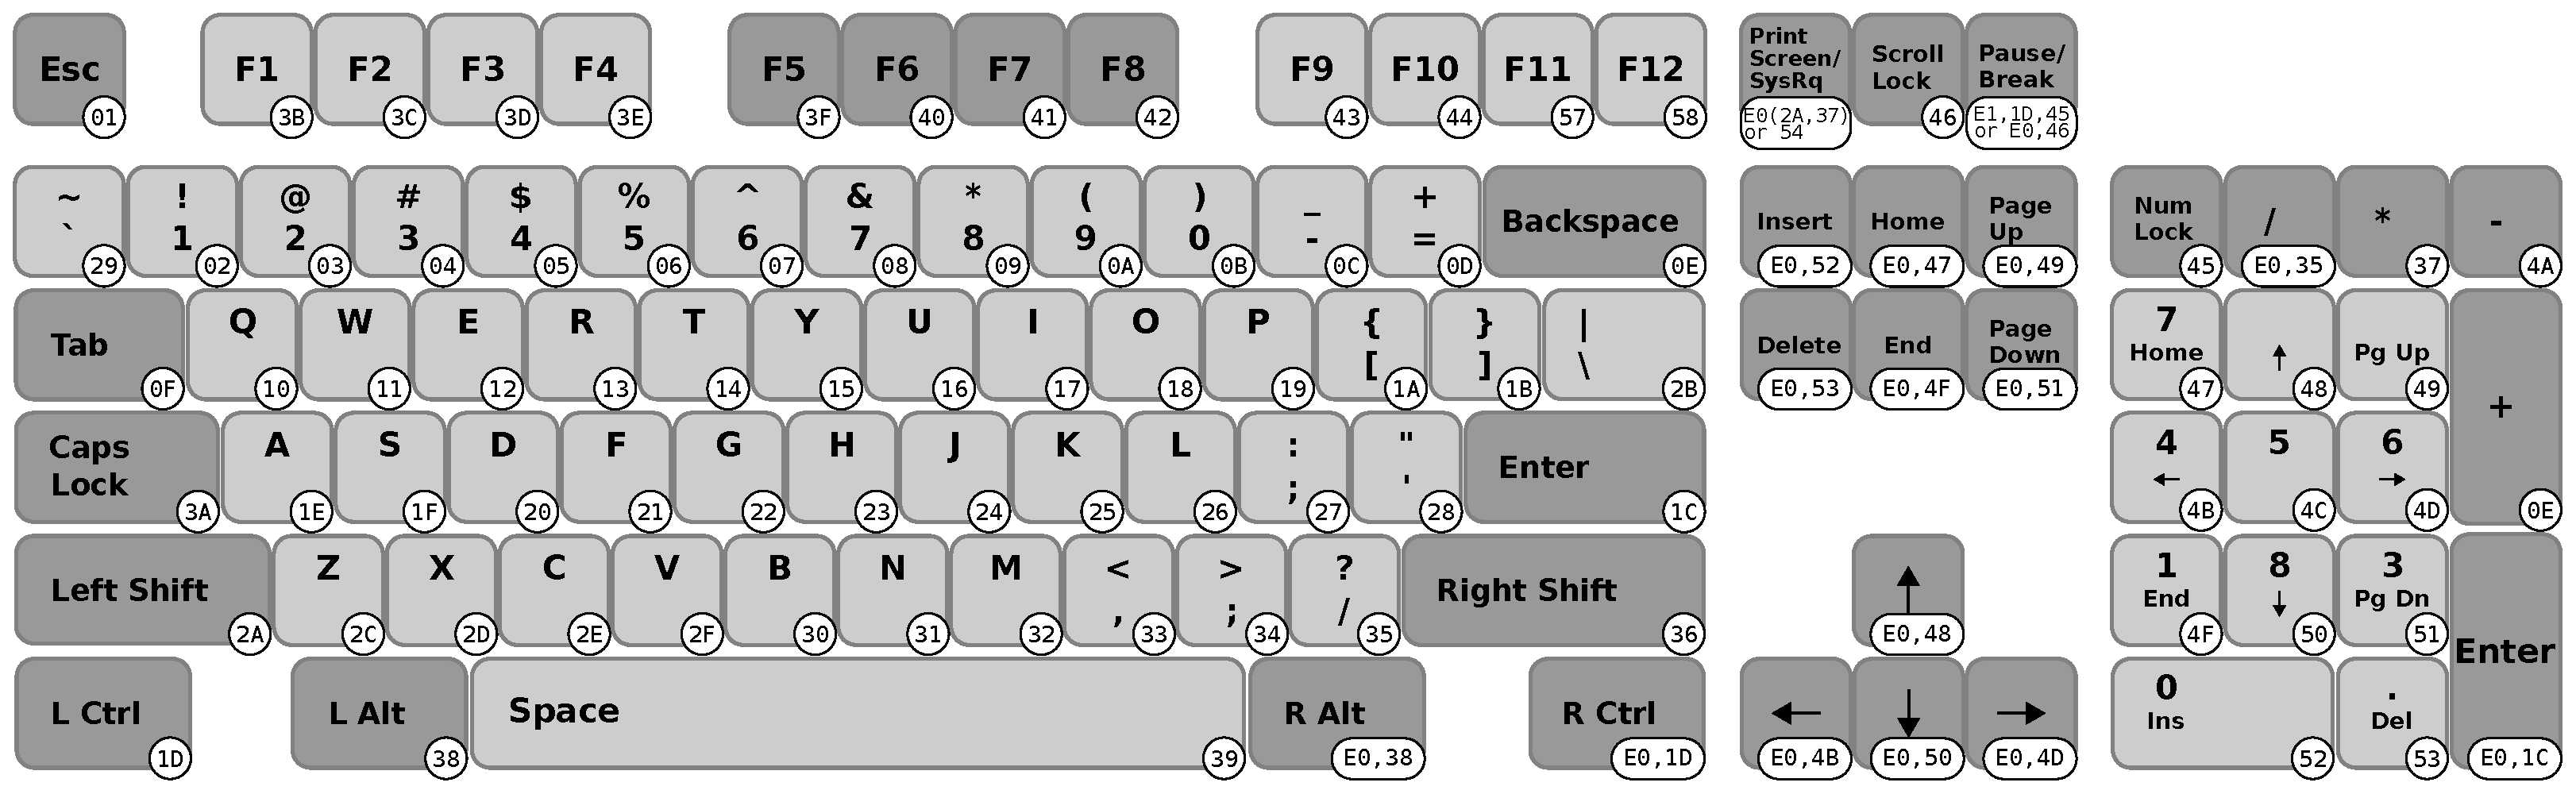
\includegraphics[width=1.0\textwidth]{imgs/drawings/keyboard_model_M.eps}
      \caption{IBM Keyboard Model M scancode layout (scancodes in hexadecimal).}
\end{figure}

\par
The Model M includes 14 keys, such as "\textbf{Right Ctrl}", "\textbf{Right Alt}", and the arrow keys, that duplicate functions from the 84-key layout. To save encoding space, these keys are sent as two-byte scancodes: the first byte is always \cw{E0h}, followed by the make or break code of the equivalent key from the original AT layout. For instance, the standard "\textbf{/}"-key produces the scancode \cw{35h}, while the numeric keypad's "\textbf{Num /}"-key sends \cw{E0h} followed by \cw{35h}. This allows software to differentiate between the keys without expanding the scancode table.\\

\par
This encoding also has the additional benefit that, if the underlying software only understands the 84-key layout, it will (presumably) discard the \cw{E0h} byte in this example and only process the \cw{35h} byte. This would result in a "\textbf{/}" being correctly typed from the numeric keypad, even though the software doesn't understand that this key exists.\\

\trivia{The \cw{E0h} scancode introduced some unexpected behaviors. For example, typing "\textbf{Shift}" + "\textbf{Num /}" should produce a "\textbf{/}", as indicated on the keycap. However, older software may interpret this sequence incorrectly: Shift is down, I don't understand \cw{E0h}, and here comes \cw{35h}. That means the user wanted to type "\textbf{?}".}



\subsection{Keyboard input}
Once a key is pressed or released, the scancode is decoded and processed by the keyboard controller. On the IBM XT, this is an Intel 8255 PPI\footnote{Programmable Peripheral Interface} chip. Its main purpose is to listen for serial data from the keyboard, verify that it arrived intact, store each incoming scancode in a buffer, and request an interrupt so it can be read by the software.\\

\par
With the advent of the IBM AT and the need for bidirectional communication with the keyboard for features like keyboard status LEDs, the Intel 8042 UPI\footnote{Universal Peripheral Interface.} chip was introduced. The UPI retained backward compatibility with the PPI chip, handling all scancodes from the keyboard. When a key is pressed, the interrupt is routed to ISR \#9 in the Vector Interrupt Table. The engine installs its own ISR there.\\

\par
\begin{figure}[H]
  \centering
  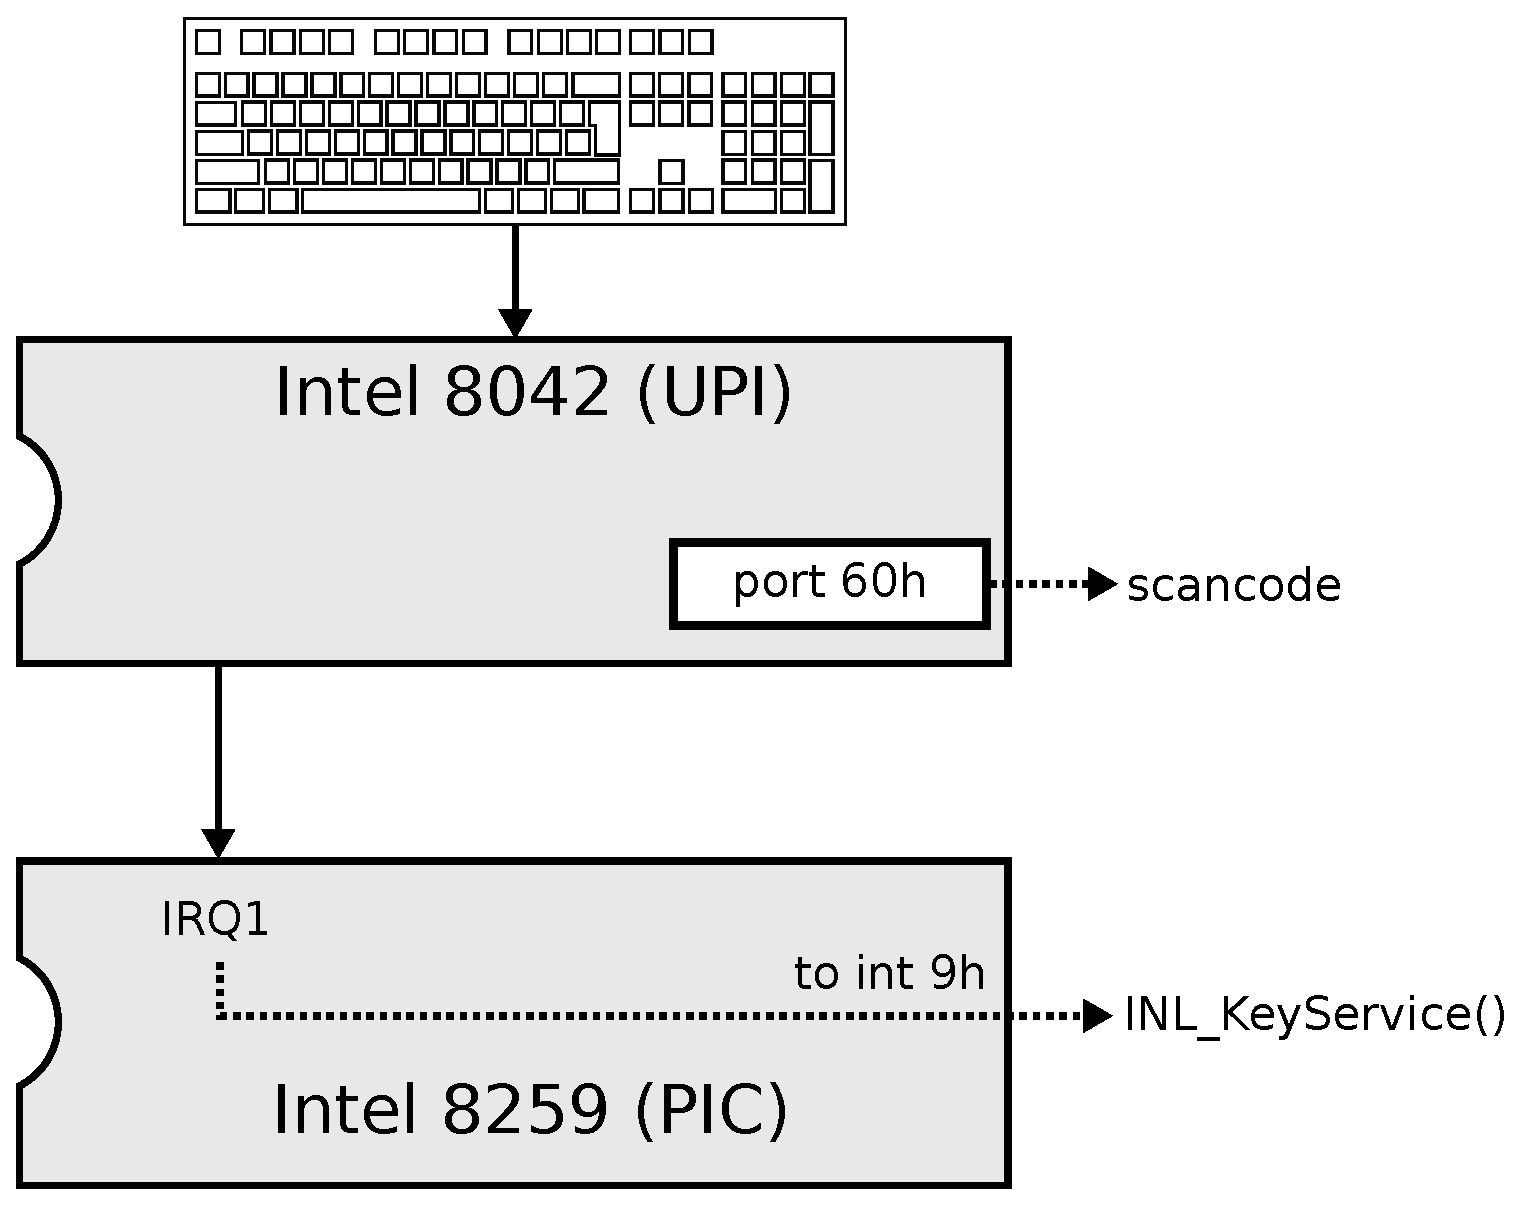
\includegraphics[width=0.8\textwidth]{imgs/drawings/keyboard.eps}
  \caption{Keyboard hardware diagram.}
  \label{fig:pc_keyboard}
\end{figure}

\par
\begin{minipage}{\textwidth}
\lstinputlisting[language=C]{code/keyboard_service.c}
\end{minipage}

\par
The state of the keyboard is maintained in a global array \cw{Keyboard}, available for the entire engine to lookup.\\
\par
\begin{minipage}{\textwidth}
\lstinputlisting[language=C]{code/keyboard_array.c}
\end{minipage}

\par
When a scancode byte arrives from the keyboard, it is copied to a buffer in the keyboard controller and an IRQ \#1 is raised. Scancodes arrive one byte at a time, and one interrupt at a time, even if it is a multi-byte code. The interrupt handler can read a byte from I/O port \cw{60h} to capture the scancode for further processing. Once that is complete, the interrupt handler must explicitly acknowledge the IRQ at the interrupt controller to re-arm it for the next keyboard event. This is accomplished by writing an "end of interrupt" signal byte to I/O port \cw{20h}. \\

\par
There is a slight difference between the PPI and the UPI in terms of how the keyboard input buffer is managed. The PPI will hold a byte in its input buffer indefinitely until the software acknowledges that it has completed the read. The acknowledgment procedure is to briefly strobe the high bit of I/O port \cw{61h} on, then off. When this occurs, the keyboard controller resets its buffer status and resumes reading from the keyboard. The UPI simplifies this process. Reading from I/O port \cw{60h} automatically resets the buffer, eliminating the need for a separate acknowledgment. However, to maintain backward compatibility, most programs still toggle the high bit of I/O port \cw{61h}, even though this has no effect on 286-based systems.\\

\par
\begin{minipage}{\textwidth}
\lstinputlisting[language=C]{code/keyboard.c}
\end{minipage}















\end{document}